%%%%%%%%%%%%%%%%%%%%%%%%%%%%%%%%%%%%%%%%%
% University/School Laboratory Report
% LaTeX Template
% Version 3.1 (25/3/14)
%
% This template has been downloaded from:
% http://www.LaTeXTemplates.com
%
% Original author:
% Linux and Unix Users Group at Virginia Tech Wiki
% (https://vtluug.org/wiki/Example_LaTeX_chem_lab_report)
%
% License:
% CC BY-NC-SA 3.0 (http://creativecommons.org/licenses/by-nc-sa/3.0/)
%
%%%%%%%%%%%%%%%%%%%%%%%%%%%%%%%%%%%%%%%%%

%----------------------------------------------------------------------------------------
%	PACKAGES AND DOCUMENT CONFIGURATIONS
%----------------------------------------------------------------------------------------

\documentclass{article}

\usepackage{graphicx} % Required for the inclusion of images
\usepackage{natbib} % Required to change bibliography style to APA
\usepackage{amsmath} % Required for some math elements
\usepackage{mathtools}
\usepackage[export]{adjustbox}
\usepackage{subcaption}
\usepackage{float}
\usepackage{listings}
\usepackage{minted}

\DeclarePairedDelimiter{\abs}{\lvert}{\rvert}
\setlength\parindent{0pt} % Removes all indentation from paragraphs

\renewcommand{\labelenumi}{\alph{enumi}.} % Make numbering in the enumerate environment by letter rather than number (e.g. section 6)

%\usepackage{times} % Uncomment to use the Times New Roman font

%----------------------------------------------------------------------------------------
%	DOCUMENT INFORMATION
%----------------------------------------------------------------------------------------

\title{ECE 637 Digital Image Processing Laboratory: \\ Pointwise Operations and
Gamma} % Title

\author{Yang \textsc{Wang}} % Author name

\date{\today} % Date for the report

\begin{document}

\maketitle % Insert the title, author and date

% If you wish to include an abstract, uncomment the lines below
% \begin{abstract}
% Abstract text
% \end{abstract}

% If you have more than one objective, uncomment the below:
%\begin{description}
%\item[First Objective] \hfill \\
%Objective 1 text
%\item[Second Objective] \hfill \\
%Objective 2 text
%\end{description}

%\subsection{Definitions}
%\label{definitions}
%\begin{description}
%\item[Stoichiometry]
%The relationship between the relative quantities of substances taking part in a reaction or forming a compound, typically a ratio of whole integers.
%\item[Atomic mass]
%The mass of an atom of a chemical element expressed in atomic mass units. It is approximately equivalent to the number of protons and neutrons in the atom (the mass number) or to the average number allowing for the relative abundances of different isotopes.
%\end{description}

%----------------------------------------------------------------------------------------
%	SECTION 1
%----------------------------------------------------------------------------------------

\section{Histogram of an Image}
	In this section, original sample images and their histograms are plotted.

\subsection{Plot Sample Images and Its Histograms}
	\begin{figure}[h]
		\begin{subfigure}{0.5\textwidth}
			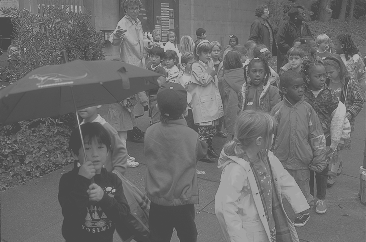
\includegraphics[width=0.9\textwidth]{kids.png}
			\caption{Original kids.tif}
		\end{subfigure}
		\begin{subfigure}{0.5\textwidth}
			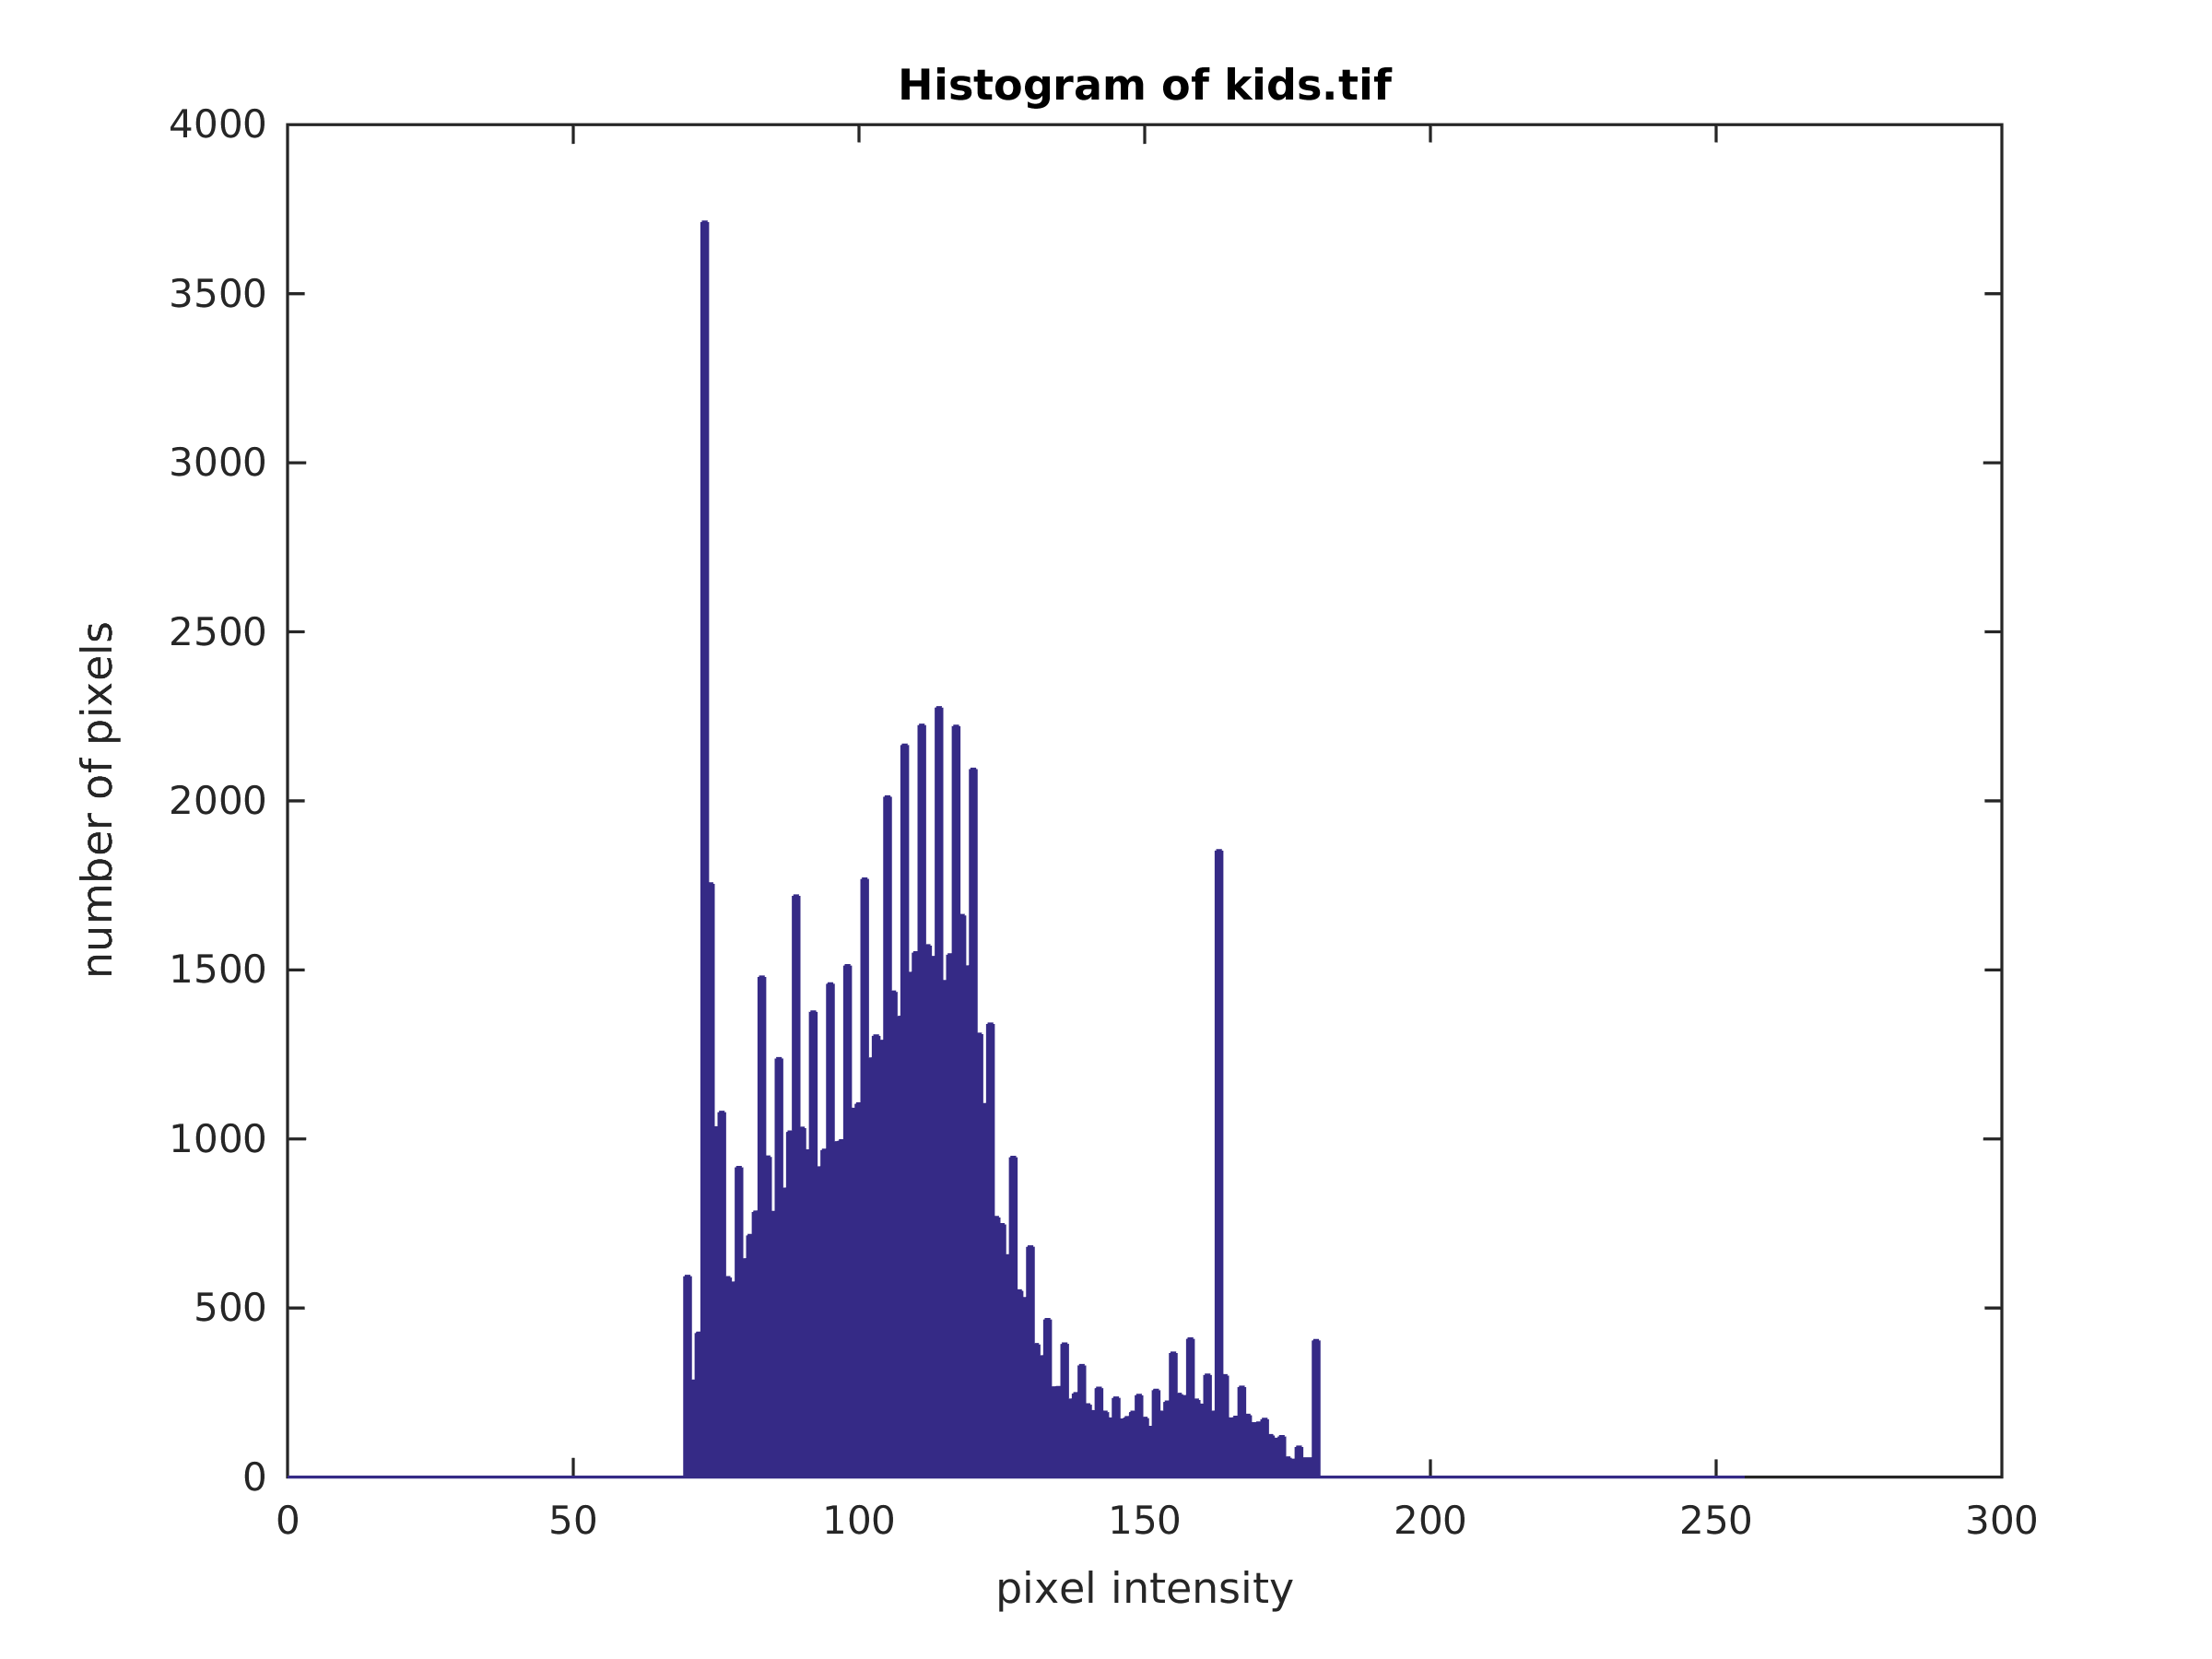
\includegraphics[width=0.9\textwidth]{kids_hist.png}
			\caption{Histogram of kids.tif}
		\end{subfigure}
	\end{figure}
	\begin{figure}[h]
		\begin{subfigure}{0.5\textwidth}
			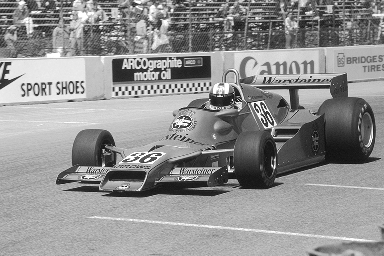
\includegraphics[width=0.9\textwidth]{race.png}
			\caption{Original race.tif}
		\end{subfigure}
		\begin{subfigure}{0.5\textwidth}
			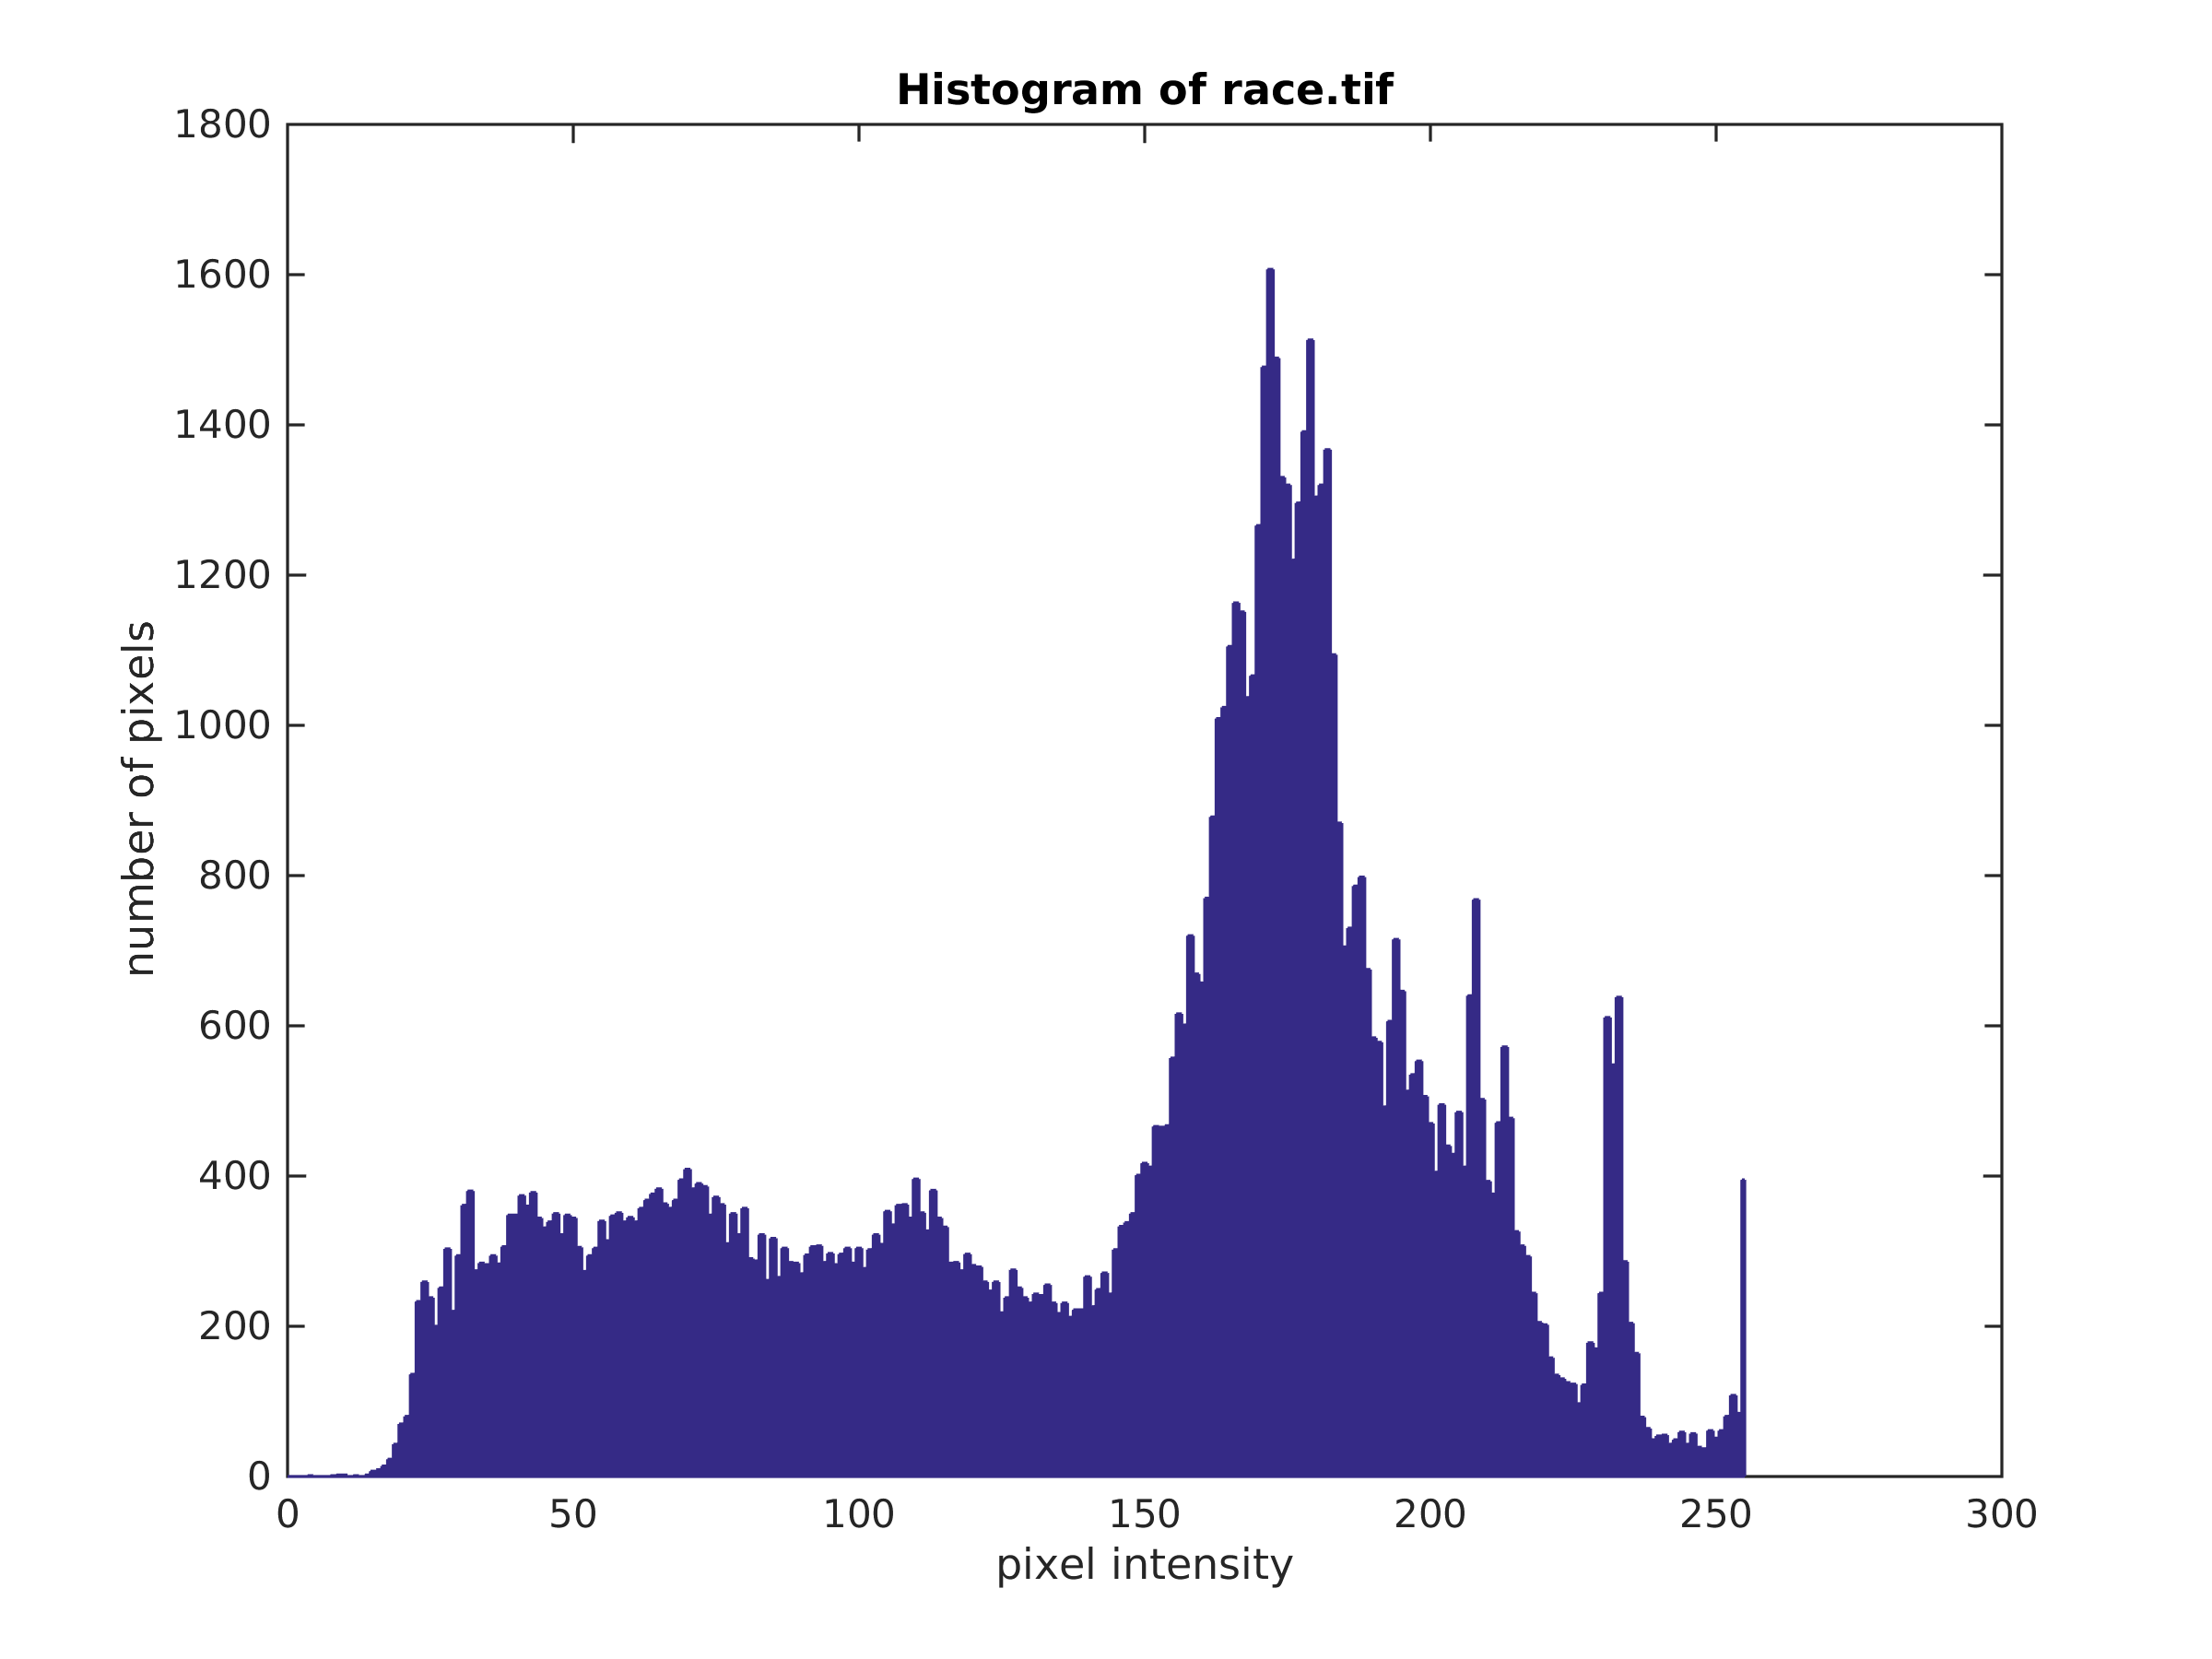
\includegraphics[width=0.9\textwidth]{race_hist.png}
			\caption{Histogram of race.tif}
		\end{subfigure}
	\end{figure}

\pagebreak

%----------------------------------------------------------------------------------------
%	SECTION 2
%----------------------------------------------------------------------------------------
\section{Histogram Equalization}
	In this section, histogram equalization is used to enhance the given sample
	images. A MATLAB function that implements a equalization function that
	approximates a cumalative distribution function is written.

\subsection{Plot the CDF $\hat{F}_x(i)$}
	\begin{figure}[h]
		\begin{center}
			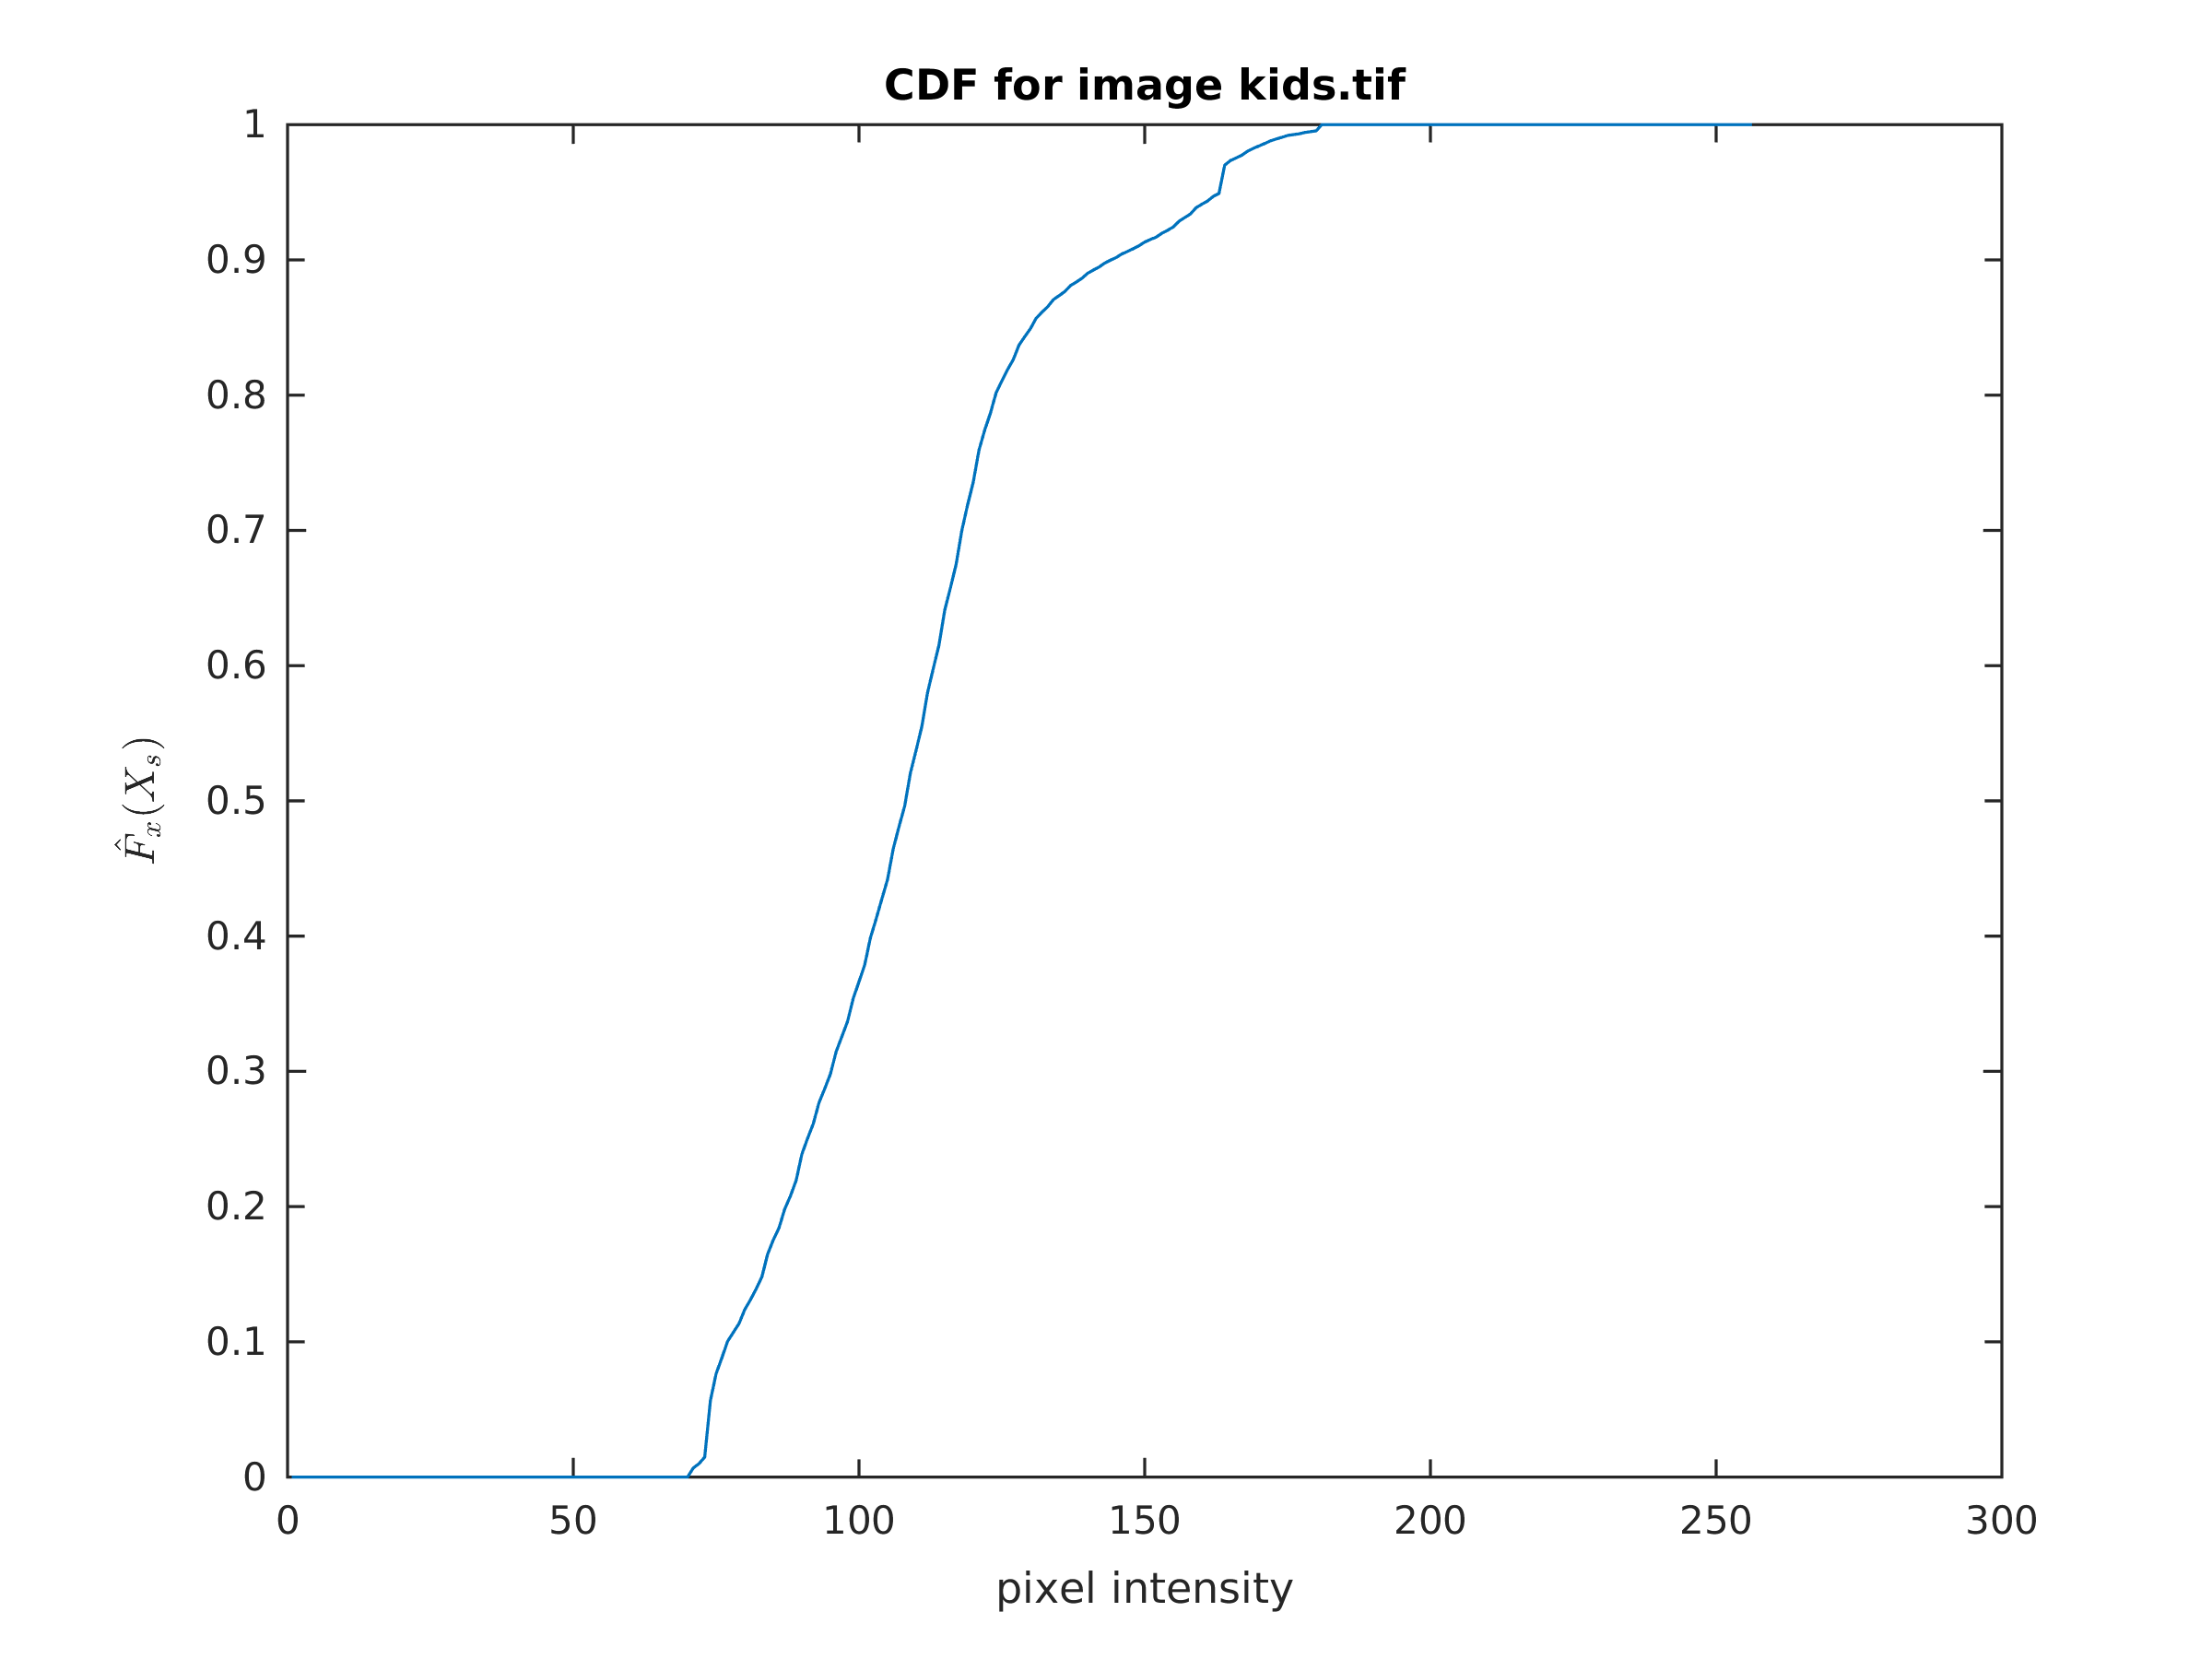
\includegraphics[width=0.6\textwidth]{kids_cdf.png}
			\caption{CDF $\hat{F}_x(i)$}
		\end{center}
	\end{figure}

\subsection{Plot the Histogram of the Equalized Image}
	\begin{figure}[h]
		\begin{center}
			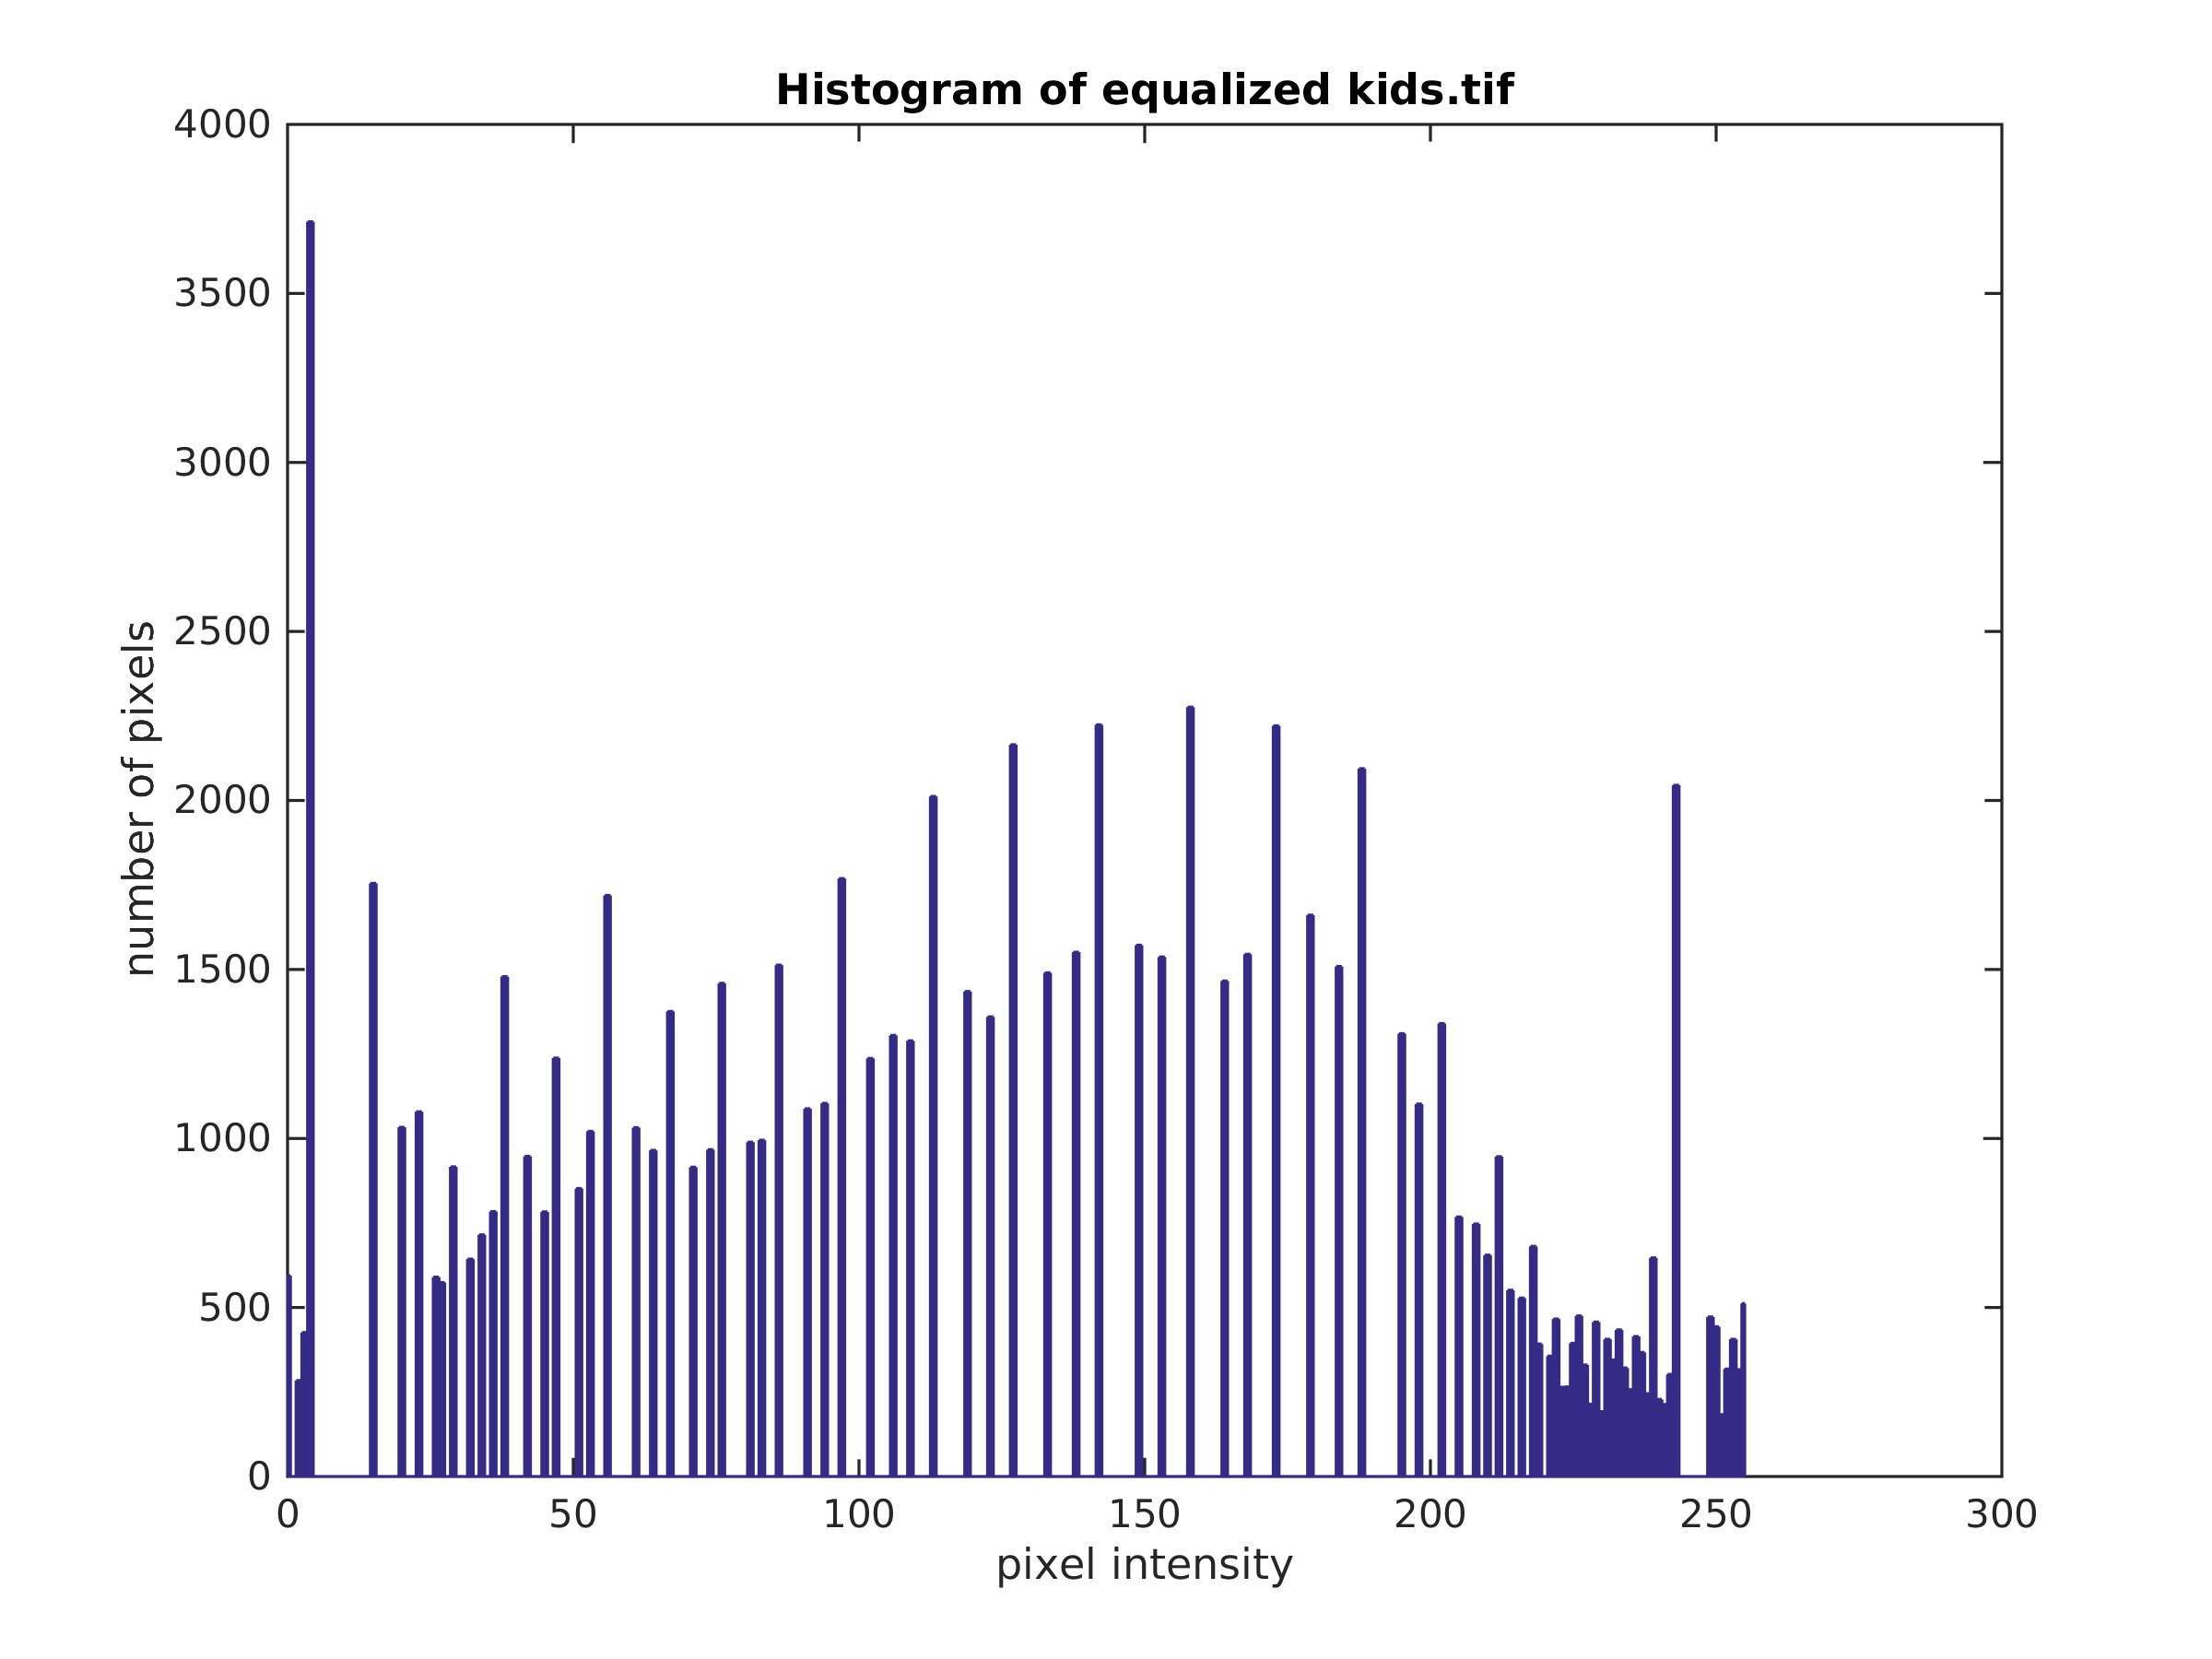
\includegraphics[width=0.6\textwidth]{kids_equ_hist.png}
			\caption{Histogram of Equalized kids.tif}
		\end{center}
	\end{figure}

\subsection{Plot the Equalized Image}
	It is apparent that the equalized image appears to be brighter than the
	original image.
	\begin{figure}[h]
		\begin{center}
			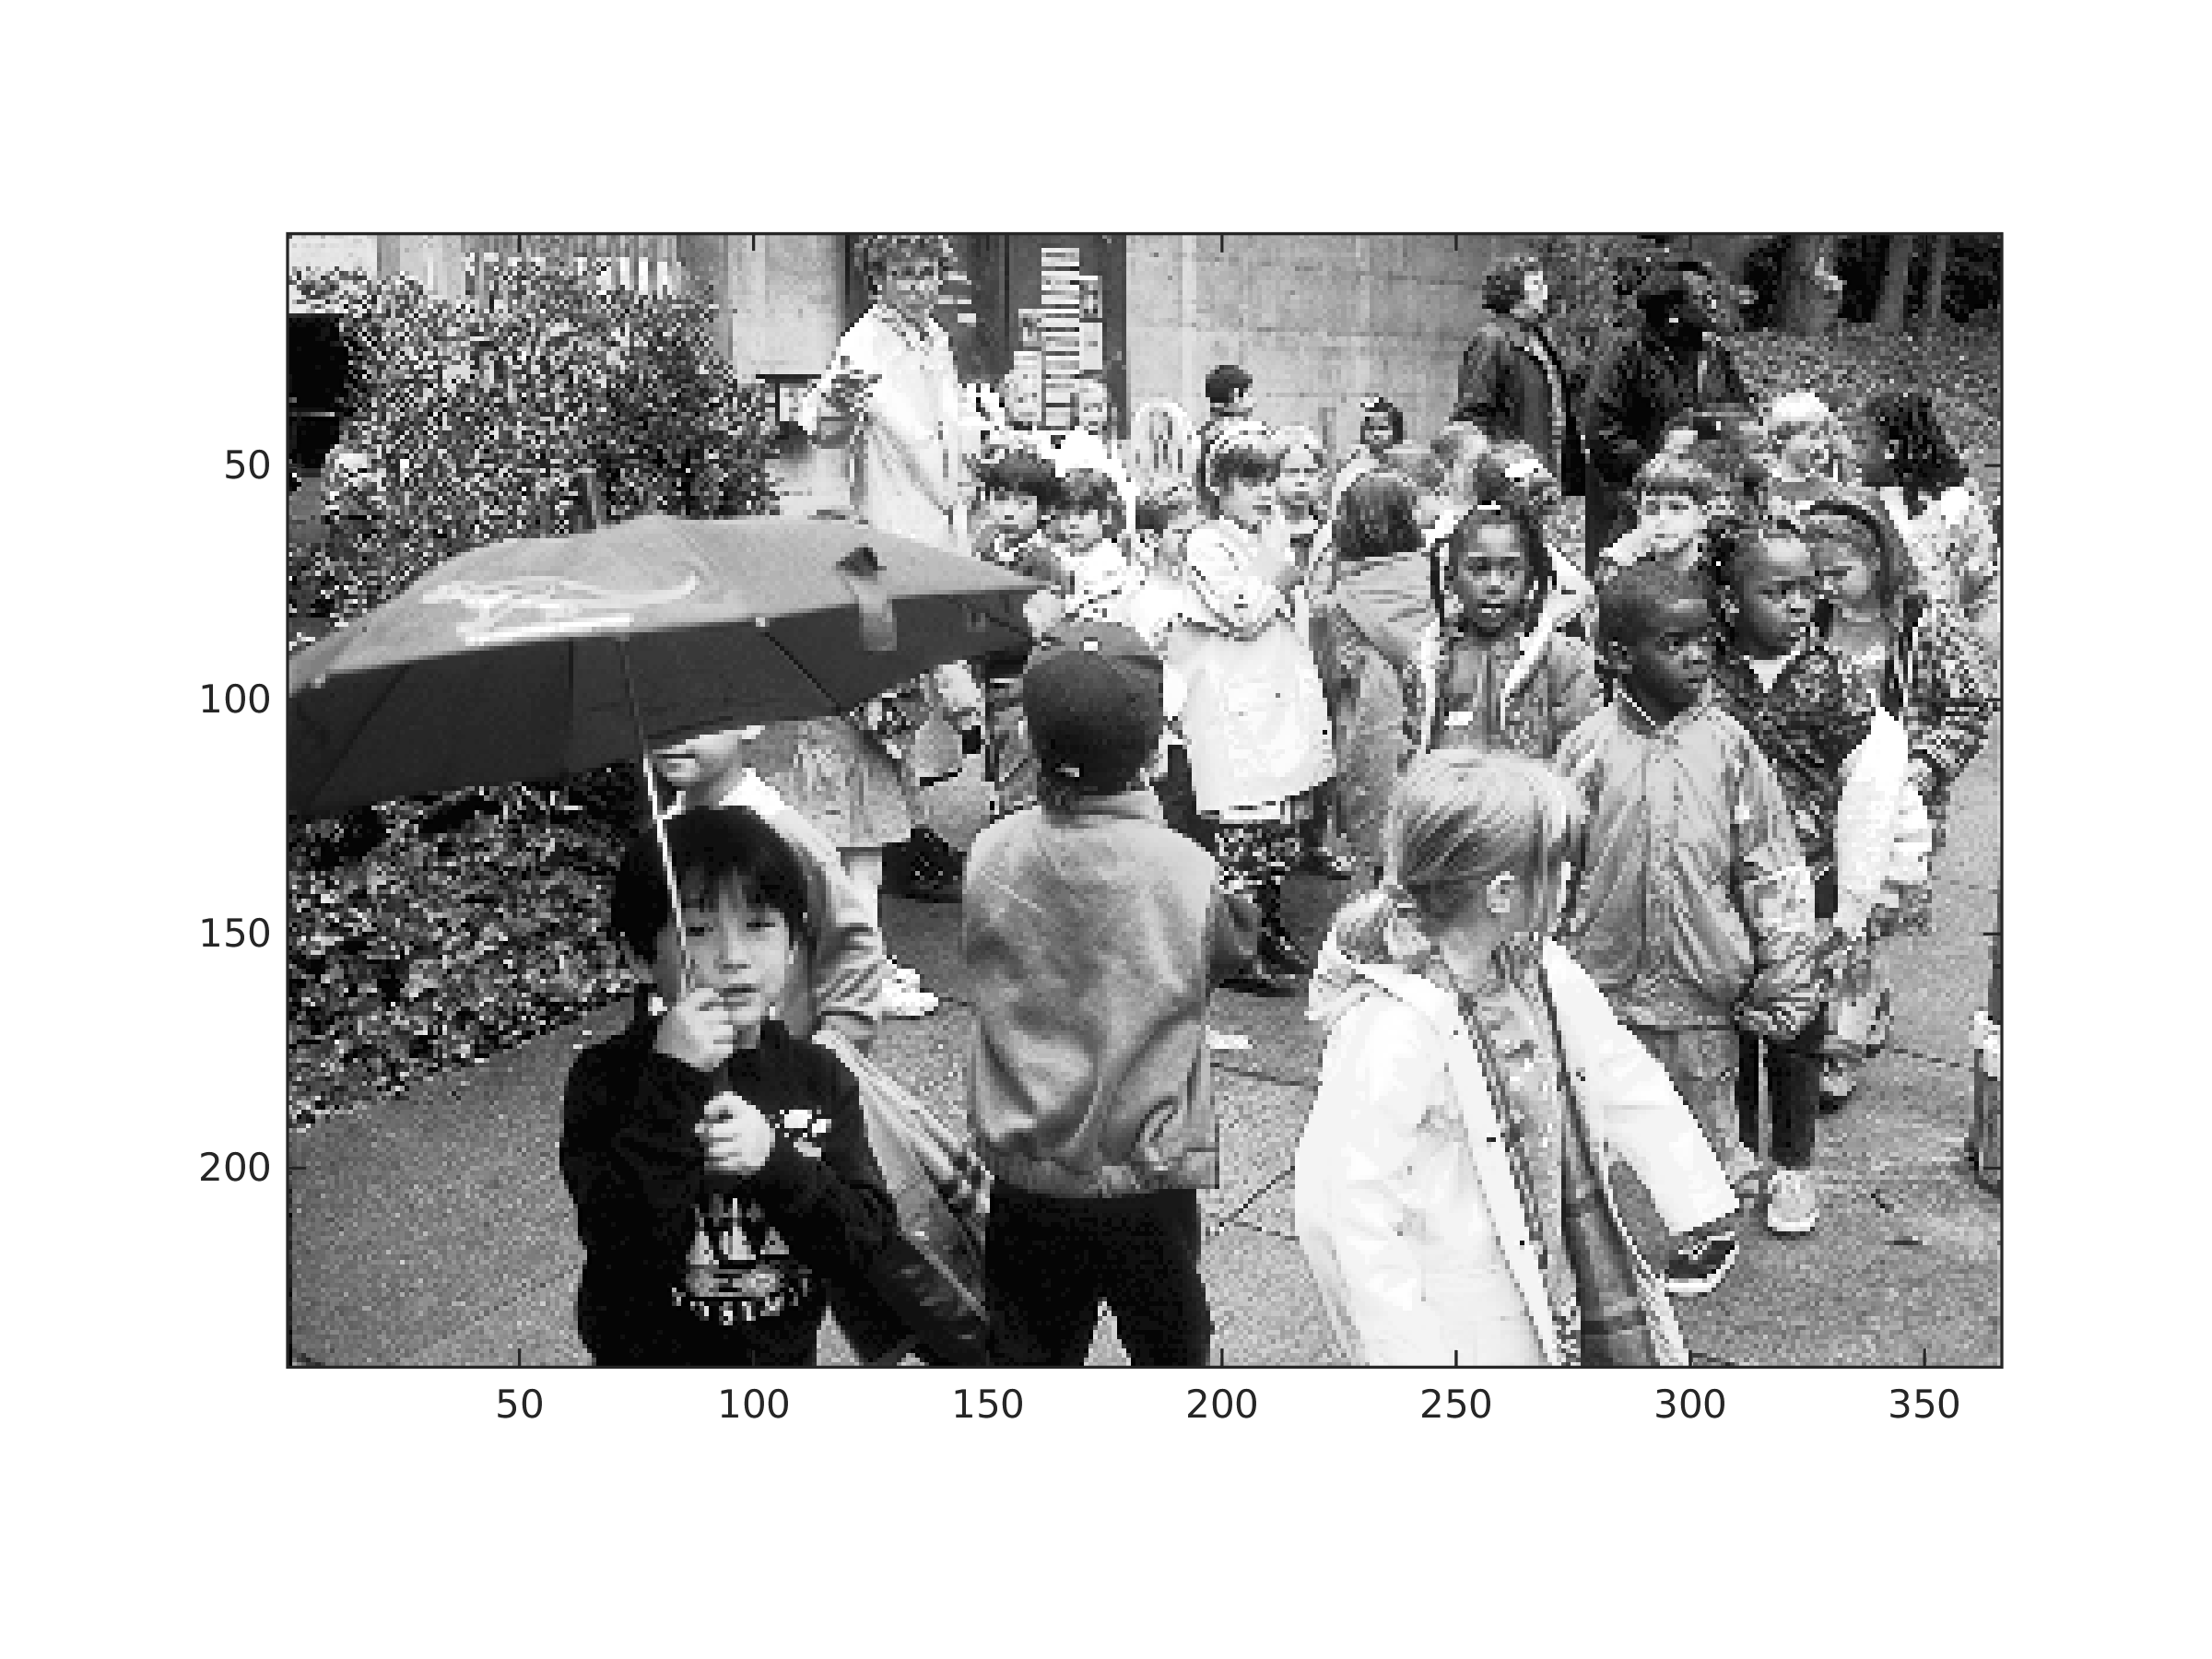
\includegraphics[width=0.6\textwidth]{kids_equ.png}
			\caption{Equalized Image of kids.tif}
		\end{center}
	\end{figure}

\subsection{Code Listing}
	\subsubsection{equalize.m}
		\inputminted[tabsize=4,breaklines]{matlab}{equalize.m}
	\subsubsection{sec1.m}
		\inputminted[tabsize=4,breaklines]{matlab}{sec1.m}

%----------------------------------------------------------------------------------------
%	SECTION 3
%----------------------------------------------------------------------------------------
\section{Contrast Stretching}
	In this section, another useful image enhancement technique called contrast
	stretching is explored. The main idea is to define two thresholds, $T1$ and
	$T2$; $T1$ has a value relatively close to 0 and $T2$ is relatively close to
	255. Anything less that $T1$ will be set to 0 and anything greater than $T2$
	will be set to 255. Pixel values in between these two values will keep the
	same.

\subsection{Plot the Transformed Image and its Histogram}
	\begin{figure}[h]
		\begin{subfigure}{0.5\textwidth}
			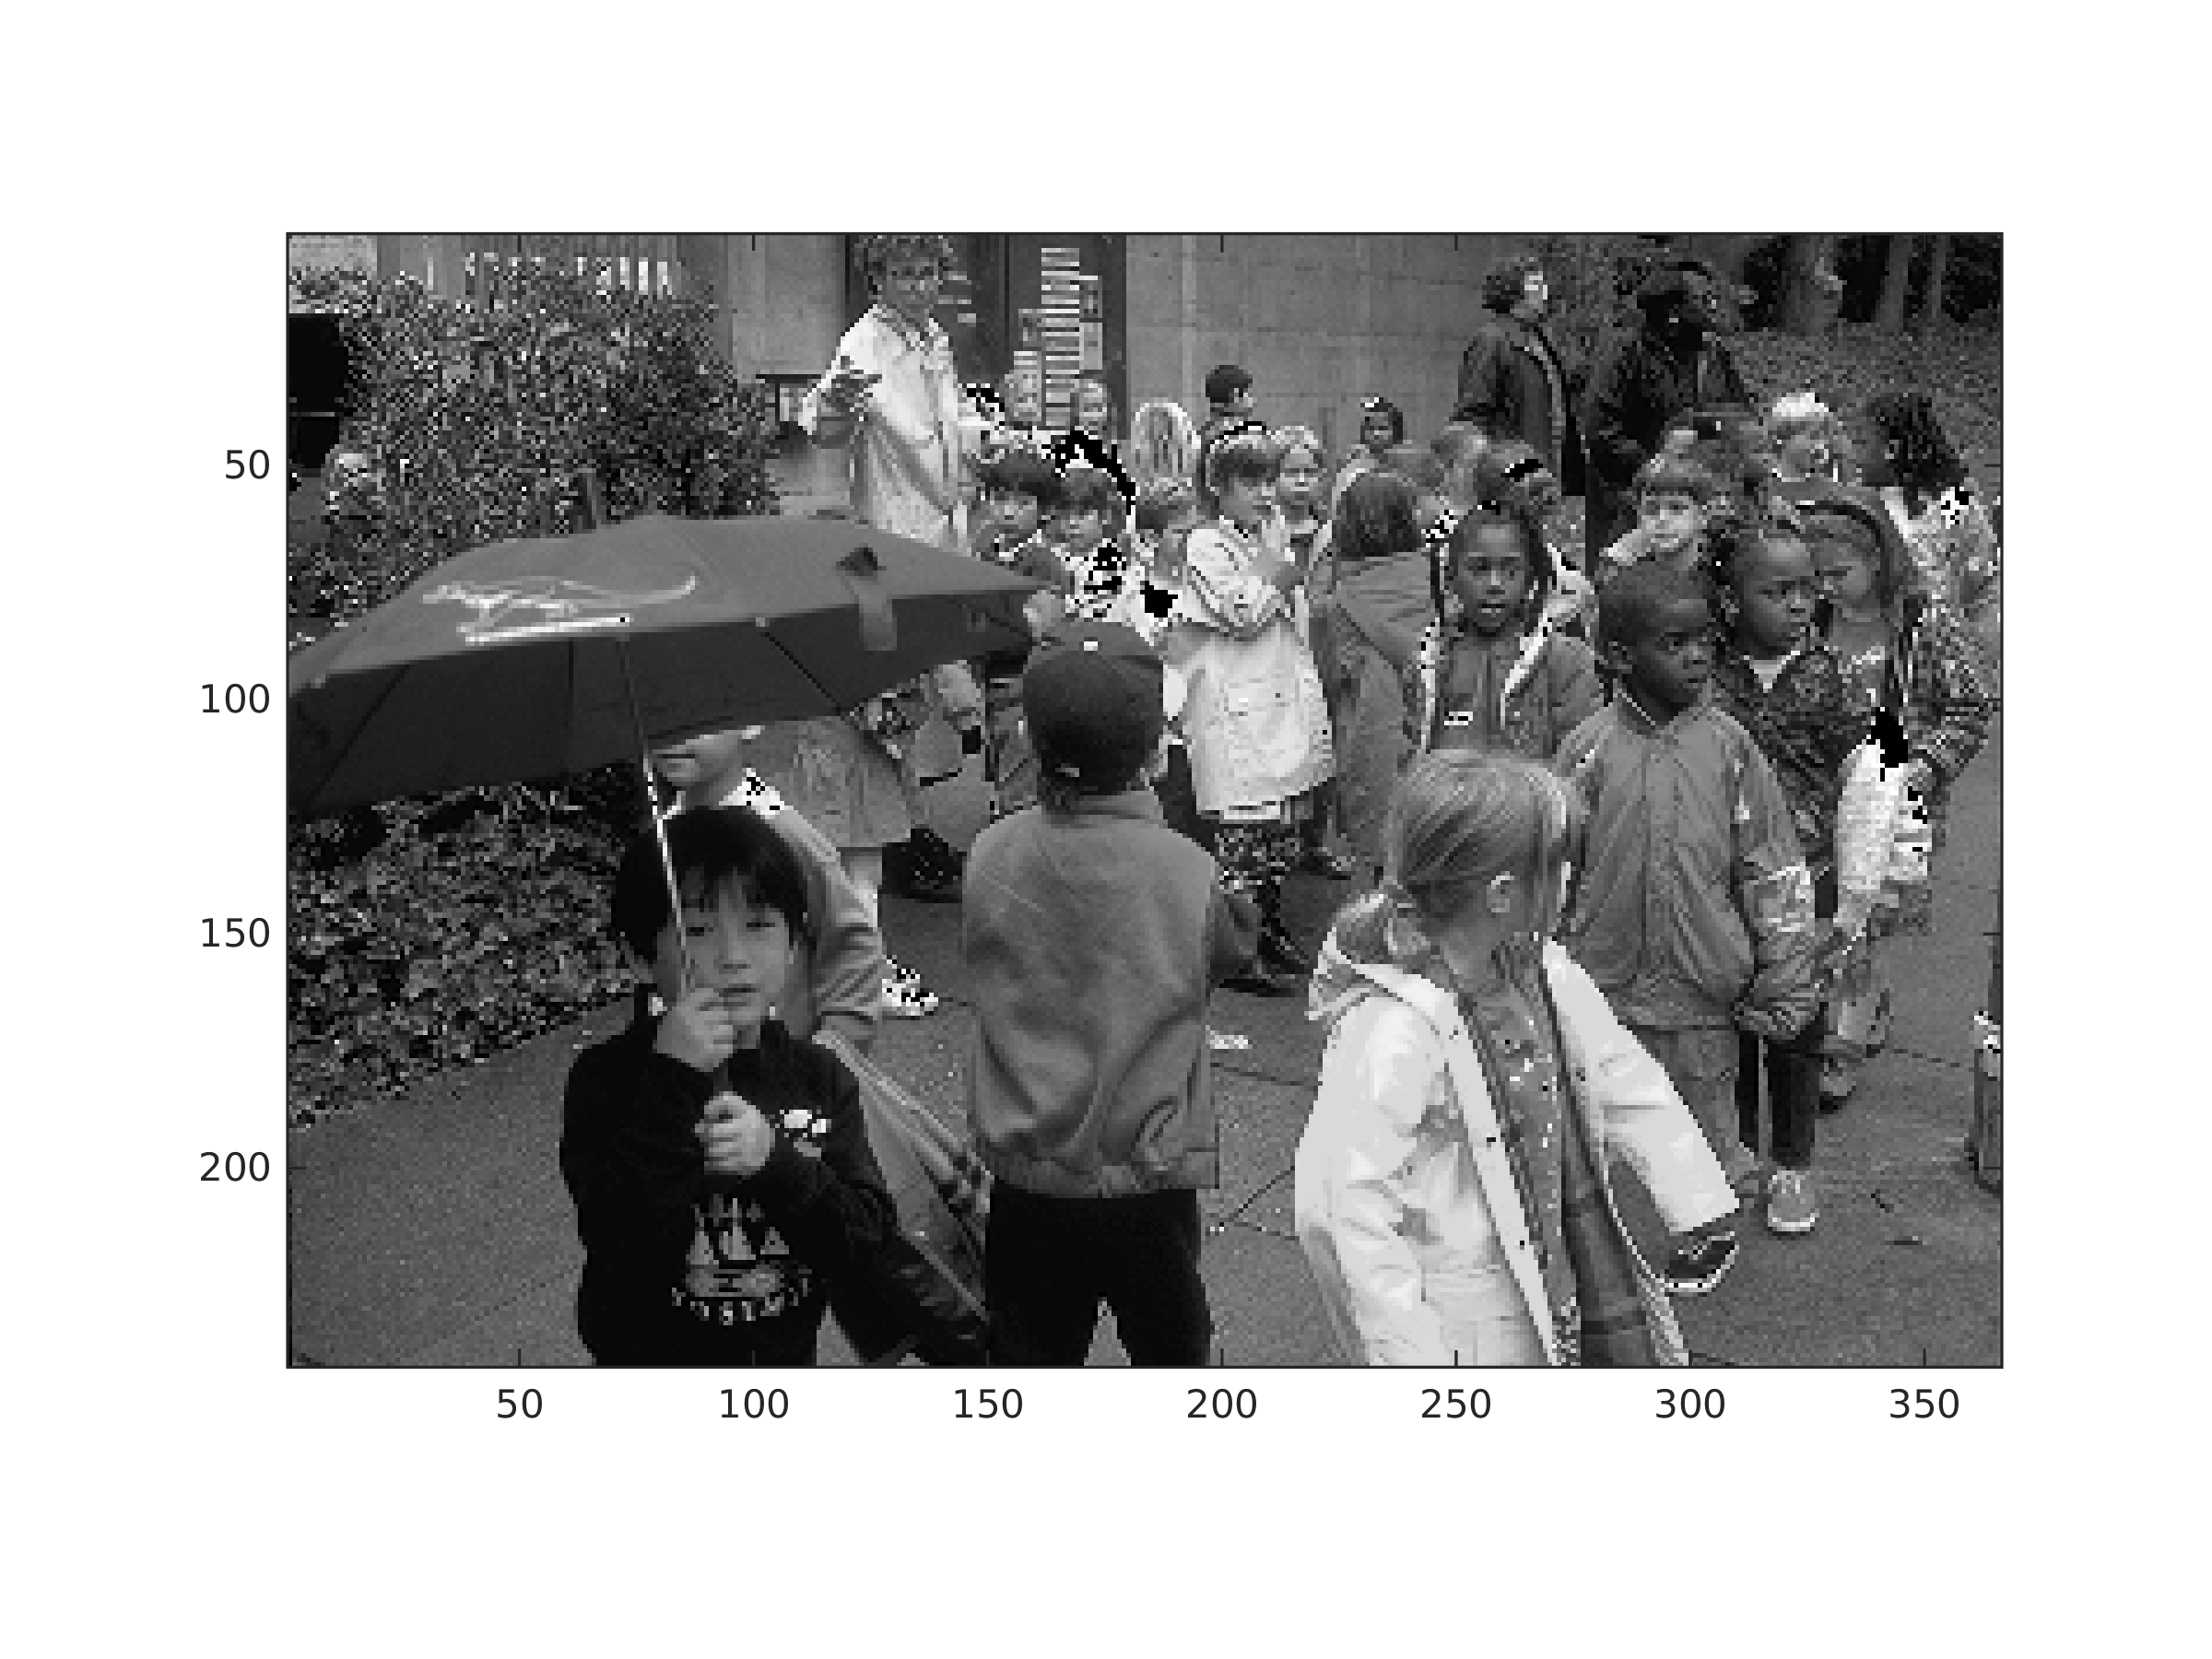
\includegraphics[width=0.9\textwidth]{kids_str.png}
			\caption{``Stretched'' kids.tif}
		\end{subfigure}
		\begin{subfigure}{0.5\textwidth}
			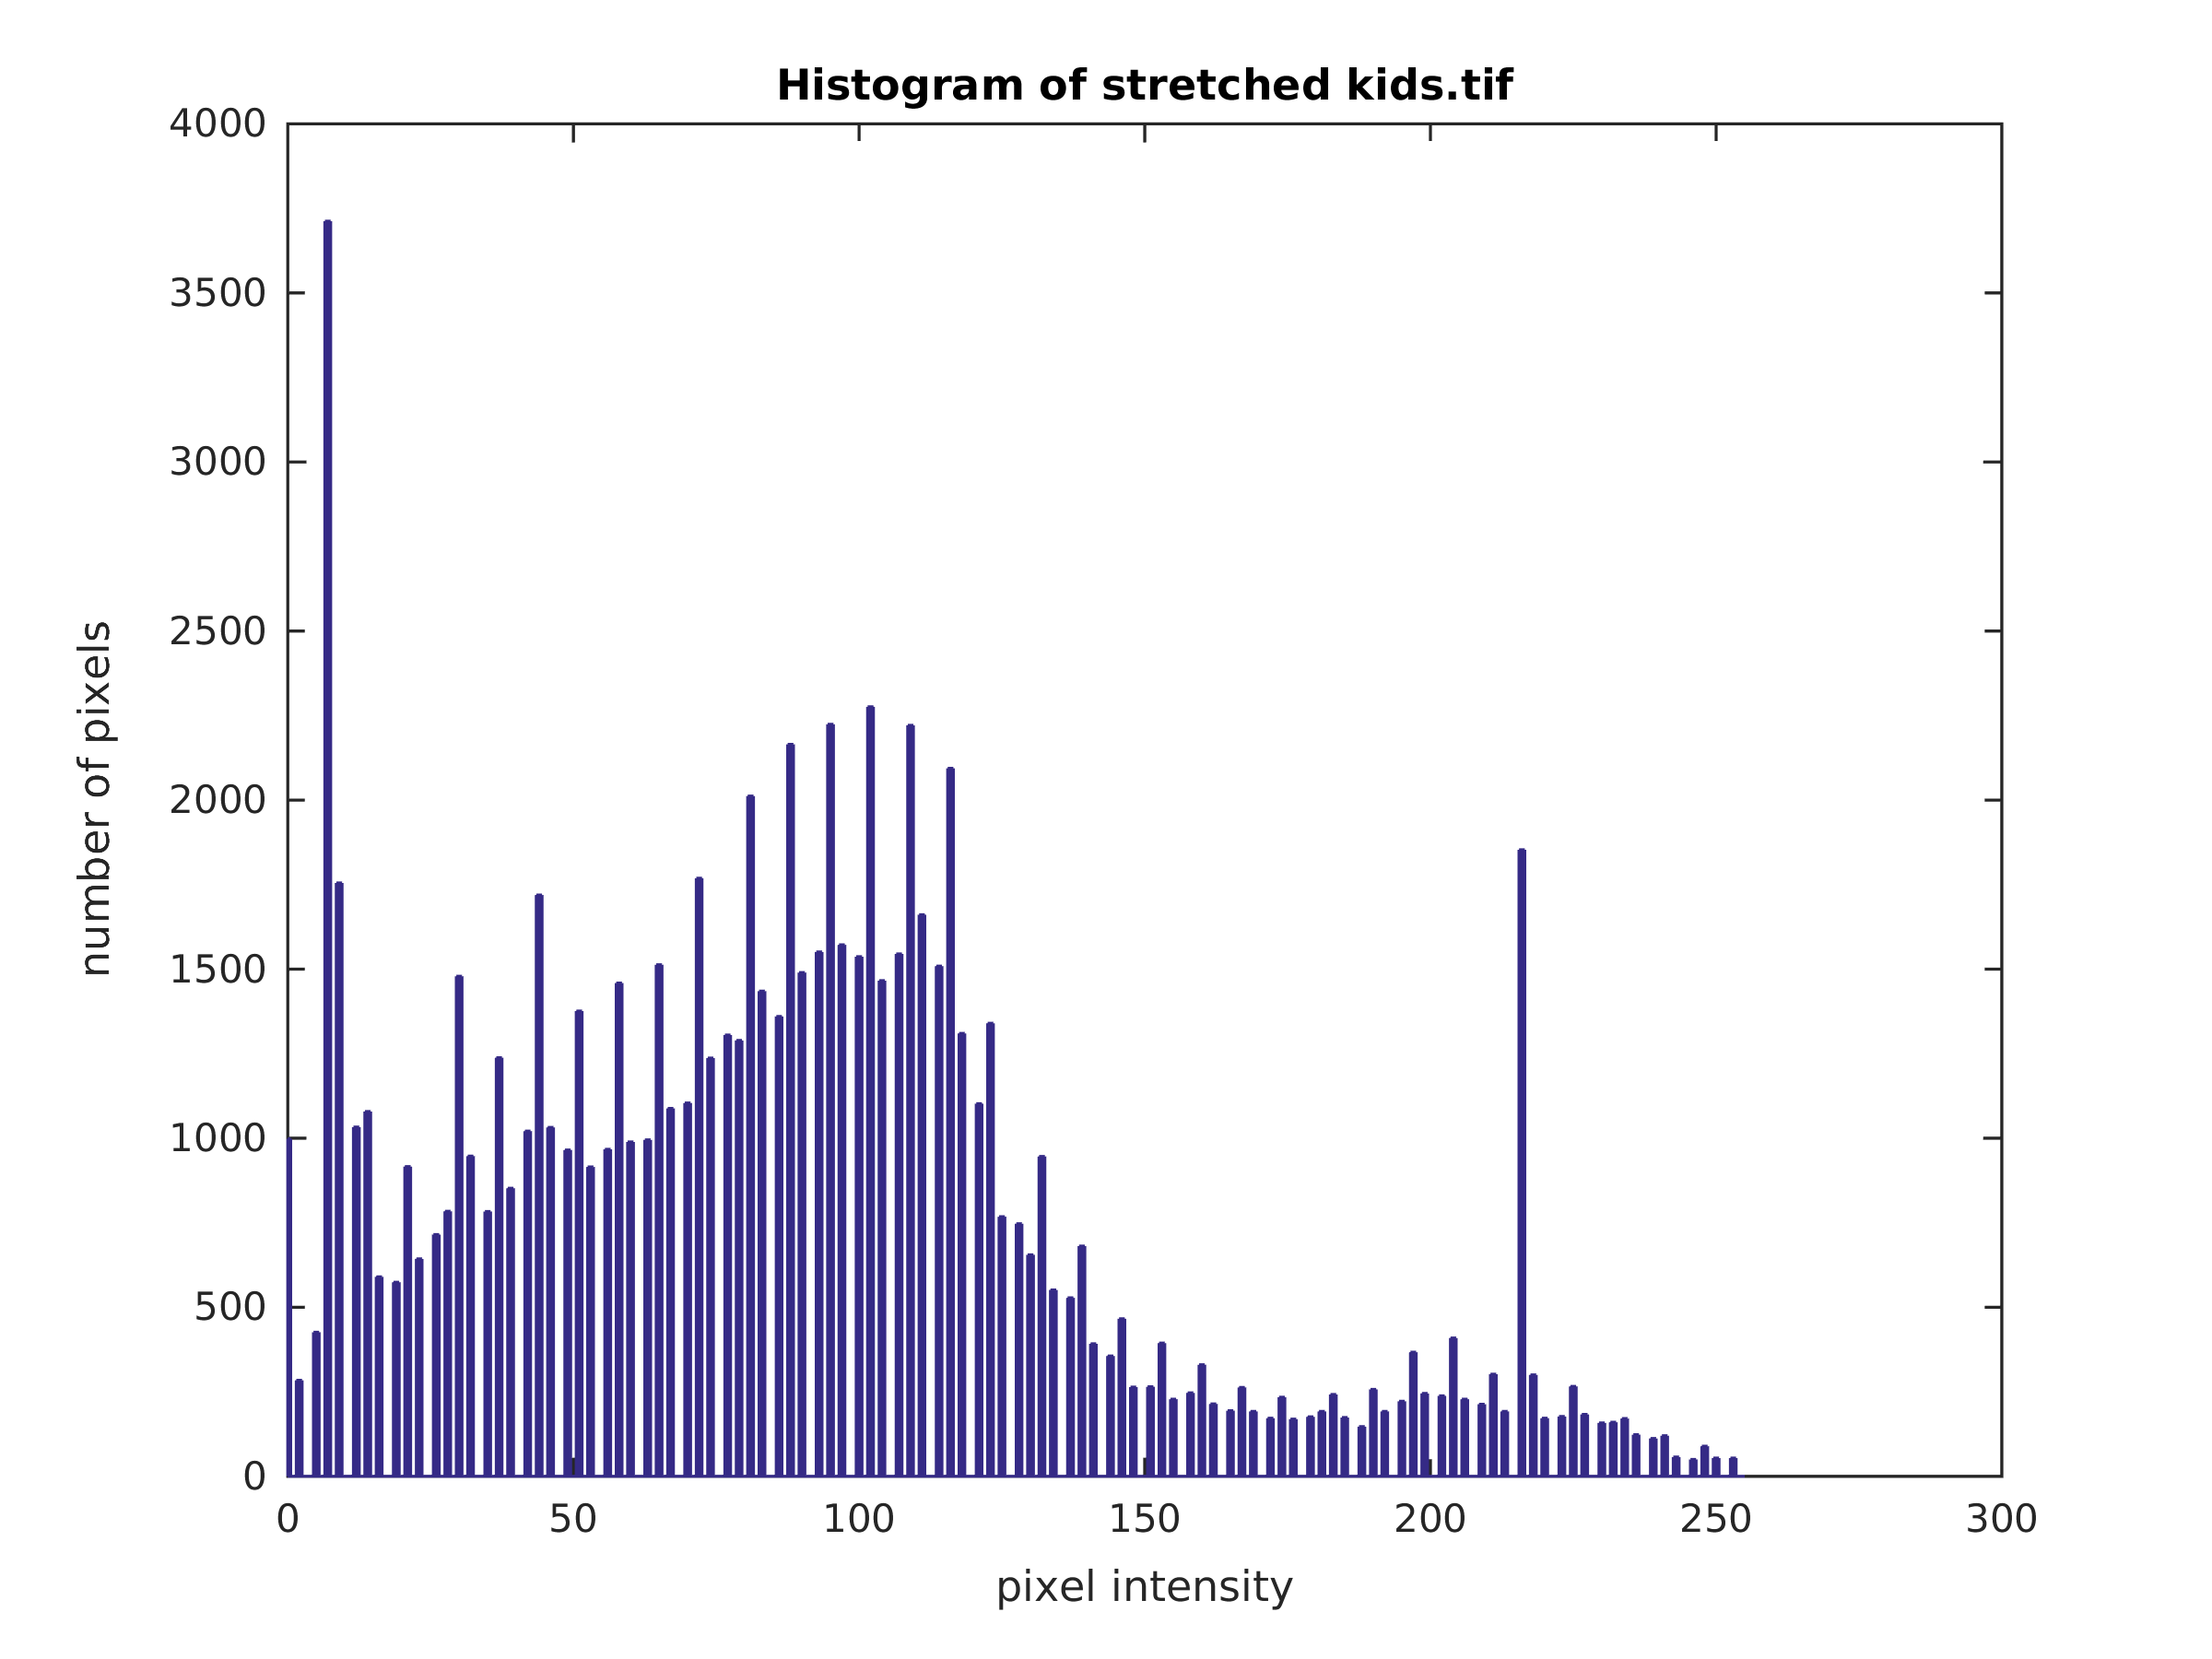
\includegraphics[width=0.9\textwidth]{kids_str_hist.png}
			\caption{Histogram of ``stretched'' kids.tif}
		\end{subfigure}
	\end{figure}

\subsection{Code Listing}
	\subsubsection{stretch.m}
		\inputminted[tabsize=4,breaklines]{matlab}{stretch.m}
	\subsubsection{sec3.m}
		\inputminted[tabsize=4,breaklines]{matlab}{sec3.m}

%----------------------------------------------------------------------------------------
%	SECTION 4
%----------------------------------------------------------------------------------------
\section{Gamma ($\gamma$)}
	In this section, the topic of gamma, gamma correction and its relation with
	gray level is discussed.

\subsection{Setting the Black Level and Picture of Your Monitor}
	Values are set. Nothing due for report.

\subsection{Determining the Gamma of Your Computer}
	\subsubsection{Plot the Checkboard to the Matching Gray Level}
		It is determined from my screen that with a gray level of 195, it
		produces the best intensity match between the stripes.

		\begin{figure}[h]
			\begin{center}
				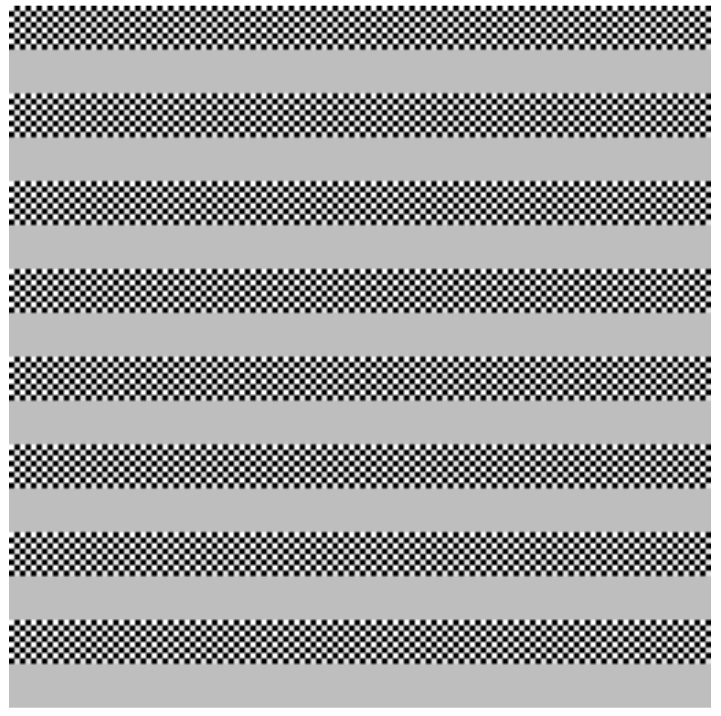
\includegraphics[width=0.6\textwidth]{checker.png}
				\caption{Checkerboard Image with gray level 195}
			\end{center}
		\end{figure}

	\subsubsection{Derive an Expression that Relates the Matching Gray Level
					to the Value of $\gamma$}
		We are given:
		\begin{align*}
			I_c = \frac{I_{255}}{2}
		\end{align*}
		and:
		\begin{align*}
			I_g = I_{255}(\frac{g}{255})^{\gamma}
		\end{align*}
		For matching gray level, we have:
		\begin{align*}
			I_c &= I_g \\
			\frac{I_{255}}{2} &= I_{255}(\frac{g}{255})^{\gamma}
		\end{align*}
		Hence,
		\begin{equation}
			\gamma = -{\frac{\log{2}}{\log{\frac{g}{255}}}}
		\end{equation}

	\subsubsection{Calculate the Value of Gray Level and $\gamma$}
		Using equation (1), $g=195$, we have:
		\begin{align*}
			\gamma &= -{\frac{\log{2}}{\log{\frac{195}{255}}}} \\
					&= 2.583
		\end{align*}

\subsection{Gamma Correction}
	\subsubsection{Plot the Original and the Corrected Images}
		\begin{figure}[h]
			\begin{subfigure}{0.5\textwidth}
				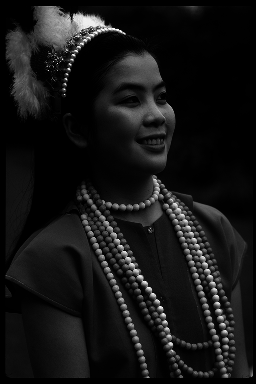
\includegraphics[width=0.9\textwidth]{linear.png}
				\caption{Original linear.tif}
			\end{subfigure}
			\begin{subfigure}{0.5\textwidth}
				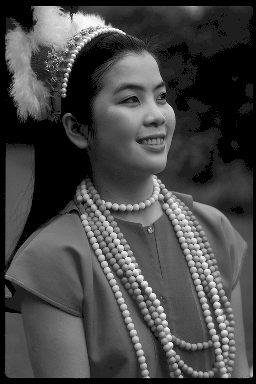
\includegraphics[width=0.9\textwidth]{linear_gamma.png}
				\caption{Corrected linear.tif with $\gamma=2.583$}
			\end{subfigure}
		\end{figure}

	\subsubsection{Derive the Formula for Transforming the Image}
		We have:
		\begin{align*}
			y &= 255(\frac{x}{255})^{\gamma} \\
			\frac{y}{255} &= (\frac{x}{255})^{\gamma} \\
			\frac{x}{255} &= (\frac{y}{255})^{\gamma}
		\end{align*}
		Hence,
		\begin{equation}
			x = 255(\frac{y}{255})^{\gamma}
		\end{equation}

\subsection{Gamma Correction on Gamma Corrected Image}
	\subsubsection{Plot the Original and the Corrected Images}
		\begin{figure}[h]
			\begin{subfigure}{0.5\textwidth}
				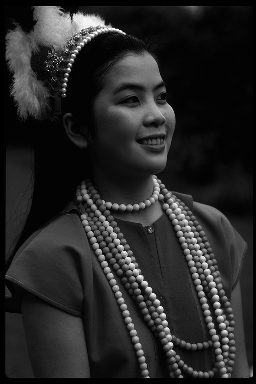
\includegraphics[width=0.9\textwidth]{gamma15.png}
				\caption{Original gamma.tif}
			\end{subfigure}
			\begin{subfigure}{0.5\textwidth}
				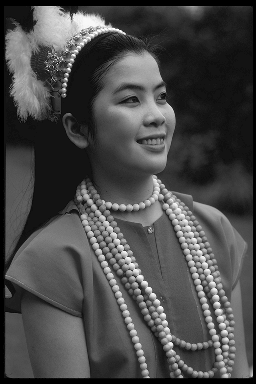
\includegraphics[width=0.9\textwidth]{gamma15_gamma.png}
				\caption{Corrected gamma.tif with $\gamma$=$\frac{1.5}{2.583}$}
			\end{subfigure}
		\end{figure}

	\subsubsection{Derive the Formula for Transforming the Image}
		Let's say we already have a image with gamma correction $\gamma_{1}$:
		\begin{align*}
			y = 255(\frac{x}{255})^{\gamma_{1}}
		\end{align*}
		And we want to do another gamma correction on top of that with
		$\gamma_{2}$,
		\begin{align*}
			z = 255(\frac{y}{255})^{\gamma_{2}}
		\end{align*}
		Then the result image will be:
		\begin{equation}
			z = 255(\frac{x}{255})^{\frac{\gamma_{1}}{\gamma_{2}}}
		\end{equation}
		Hence, for given $\gamma_{1}$ = 1.5, the resulting $\gamma$ will be:
		\begin{align*}
			\gamma = \frac{1.5}{2.583}
		\end{align*}

\subsection{Code Listing}
	\subsubsection{sec3.m}
		\inputminted[tabsize=4,breaklines]{matlab}{sec4.m}

\end{document}
